%!TEX root = ../thesis.tex
%******************************************************************************
\chapter{An Adaptive Middleware for Near-Time Processing of Bulk Data}\label{ch:adaptive_middleware}
%******************************************************************************

\section{Introduction}\label{sec:introduction}
This section introduces the concept of an adaptive middleware which is able to adapt its processing type fluently between batch processing and single-event processing. It continuously monitors the load of the system and controls the message aggregation size. Depending on the current aggregation size, the middleware automatically chooses the appropriate service implementation and transport mechanism to further optimize the processing.

In this chapter, a solution to this problem is proposed:

\begin{itemize}
	\item The concept of a middleware is presented that is able to adapt its processing type fluently between batch processing and single-event processing. By adjusting the data granularity at runtime, the system is able to minimize the end-to-end latency for different load scenarios.
\end{itemize}

The remainder of this chapter is organized as follows. Section \ref{sec:ch5_related_work} gives an overview of other work related to this research. Finally, Section \ref{sec:ch5_summary} concludes the chapter.

\section{Middleware Components}
Table \ref{table:ch4_middleware_components} shows the components of the middleware, that are based on the Enterprise Integration Patterns described by \cite{Hohpe:2003fk}.

\begin{table}[htpb]
	\caption{Components of the Adaptive Middleware. We are using the notation defined by \cite{Hohpe:2003fk}}
	\label{table:ch4_middleware_components}
	\centering
	\begin{tabular}{|m{3cm}|m{2cm}|m{5cm}|}
		\hline
		\bfseries Symbol & \bfseries Component & \bfseries Description\\
		\hline 
		\begin{center}
			
\includegraphics[scale=0.5]{message_symbol}
		\end{center} 
		& Message & A single message representing a business event.\\
		\hline 
		\begin{center}
			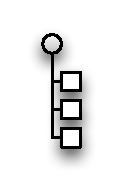
\includegraphics[scale=0.5]{aggregate_symbol} 
		\end{center}
		& Message Aggregate & A set of messages aggregated by the Aggregator component.\\
		\hline
		\begin{center}
			
\includegraphics[scale=0.5]{queue_symbol} 
		\end{center}
		& Queue & Storage component which stores messages using the \ac{FIFO} principle.\\
		\hline 
		\begin{center}
			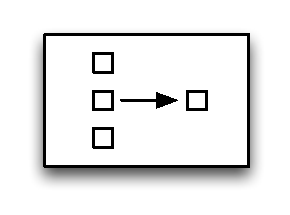
\includegraphics[scale=0.5]{aggregator_symbol}
		\end{center}
		& Aggregator & Stateful filter which stores correlated messages until a set of messages is complete and sends this set to the next processing stage in the messaging route.\\
		\hline
		\begin{center}
			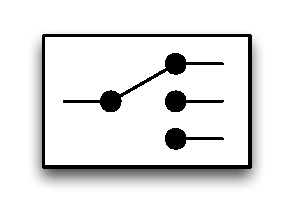
\includegraphics[scale=0.5]{router_symbol} 
		\end{center}
		& Router & Routes messages to the appropriate service endpoint.\\
		\hline
		\begin{center}
			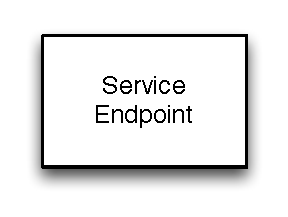
\includegraphics[scale=0.5]{endpoint_symbol} 
		\end{center}
		& Service Endpoint & Represents a business service.\\
		\hline
	\end{tabular}
\end{table}

\subsection{Aggregator}
The Aggregator is a stateful filter which stores correlated messages until a set of messages is complete and sends this set to the next processing stage in the messaging route. 

There are different options to aggregate messages, which can be implemented by the Aggregator:

\begin{itemize}
	\item \textbf{No correlation}: Messages are aggregated in the order in which they are read from the input message queue. In this case, an optimized processing is not simply possible.
	\item \textbf{Technical correlation:} Messages are aggregated by their technical properties, for example by message size or message format.
	\item \textbf{Business correlation}: Messages are aggregated by business rules, for example by customer segments or product segments.
\end{itemize}

\subsection{Feedback Loop}

To control the level of message aggregation at runtime, the middleware uses a closed feedback loop with the following properties (see Figure \ref{fig:feedback_loop}):

\begin{itemize}
	\item \textbf{Input (u):} Current aggregation size
	\item \textbf{Output (y):} Change of queue size measured between sampling intervals
	\item \textbf{Set point (r):} The change of queue size should be zero.
\end{itemize}

Ultimately, we want to control the average end-to-end latency depending on the current load of the system. The change of queue size seems to be an appropriate quantity because it can be directly measured without a lag at each sampling interval, unlike the average end-to-end latency.

\begin{figure}[htbp]
	\centering
	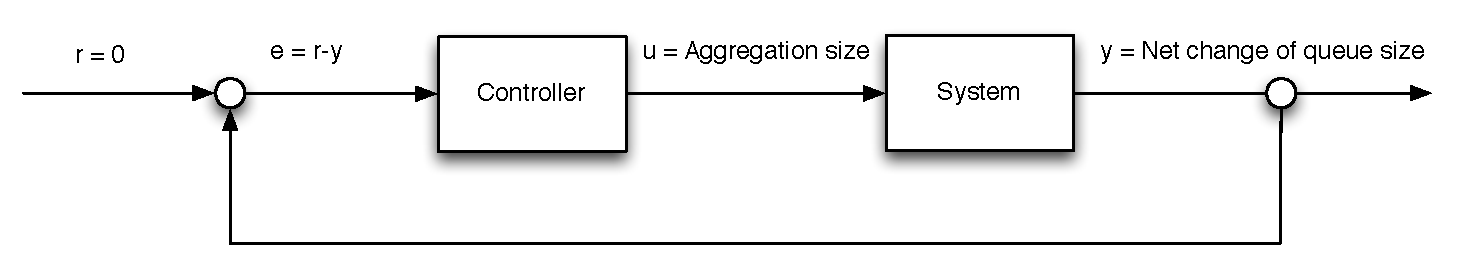
\includegraphics[width=\columnwidth]{feedback_loop}
	\caption{Feedback loop to control the aggregation size}
	\label{fig:feedback_loop}
\end{figure}
The concrete architecture and tuning of the feedback loop and the controller is subject to our ongoing research.
\subsection{Router}

\begin{itemize}
	\item{static router}
	\item{dynamic router}
\end{itemize}

Depending on the size of the aggregated message, the Router routes the message to the appropriate service endpoint, which is either optimized for batch or single event processing.

When processing data in batches, especially when a batch contains correlated data, there are multiple ways to speed up the processing:
\begin{itemize}
	\item To reduce I/O, data can be pre-loaded at the beginning of the batch job and held in memory.
	\item Storing calculated results for re-use in memory
	\item Use bulk database operations for reading and writing data
\end{itemize}

With high levels of message aggregation, it is not preferred to send the aggregated message payload itself over the message bus using Java Message Service (JMS) or SOAP. Instead, the message only contains a pointer to the data payload, which is transferred using File Transfer Protocol (FTP) or a shared database.

\section{Usage Scenarios}

\begin{itemize}
	\item different usage scenarios
	\item single aggregator, request/response integration pattern
	\begin{figure*}[htpb]
		\centering
		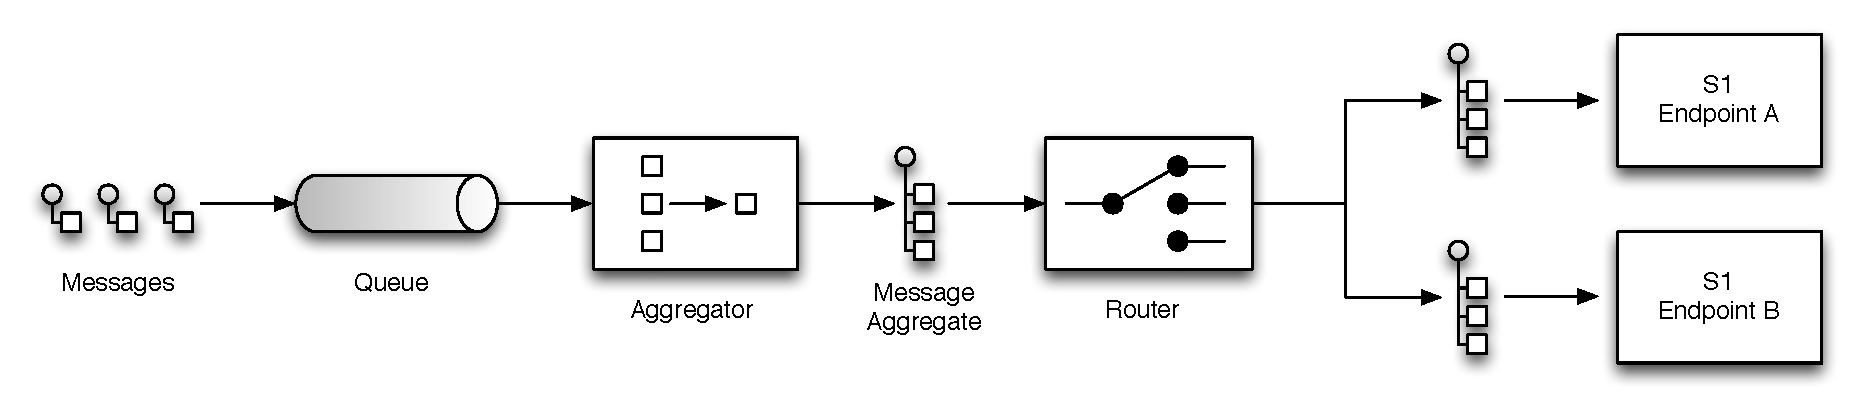
\includegraphics[width=\textwidth]{ch5_usage_scenario_1}
		\caption{single aggregator, request/response integration pattern}
		\label{fig:ch4_usage_scenario_1}
	\end{figure*}
	\item single aggregator, point to point channel
	\begin{figure*}[htpb]
		\centering
		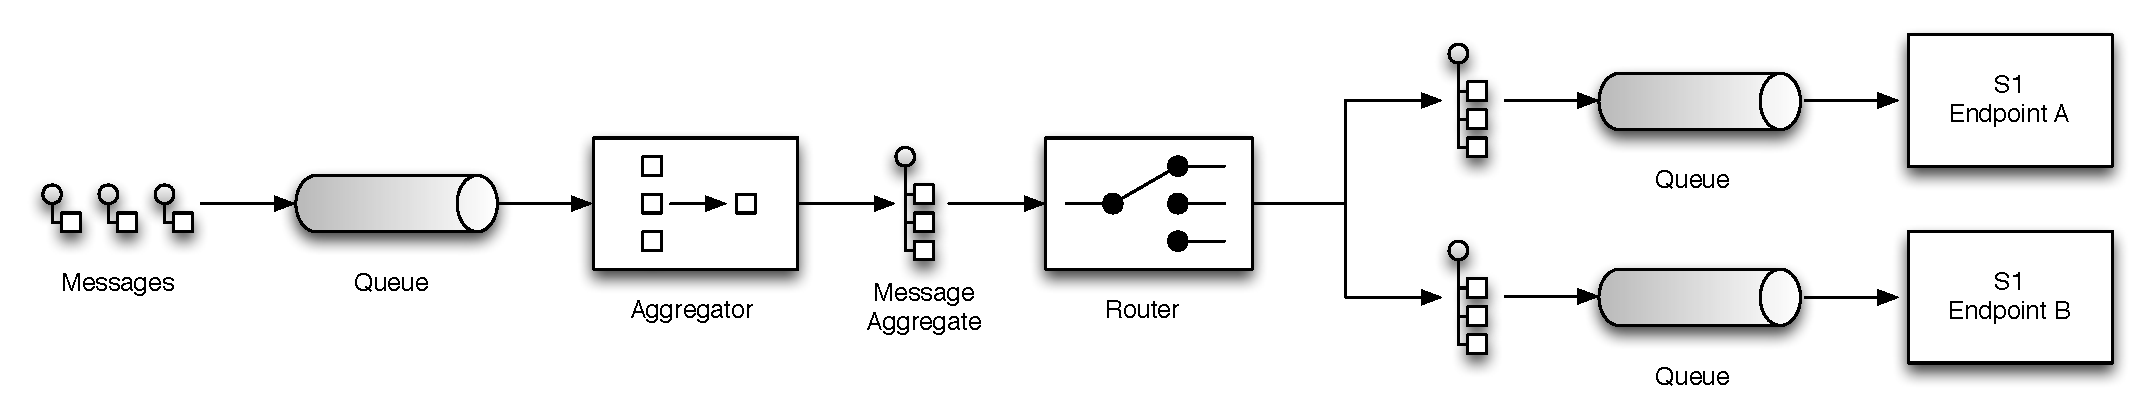
\includegraphics[width=\textwidth]{middleware_components}
		\caption{single aggregator, point to point channel}
		\label{fig:ch5_usage_scenario_2}
	\end{figure*}
	\item system consisting of multiple subsystems, with each subsystem having an input queue, aggregator, router
	
\end{itemize}	

\section{Service Design}

\begin{itemize}
	\item Services that implement the business functionality of the system need to be designed properly to support the runtime adaption between single and batch processing
	\item Service needs to support operations with a list interface
	\item Different processing algorithms for different single and batch processing
	\item Different options for service design:
	\begin{itemize}
		\item Single Service offering multiple operations for single and batch processing
		\item Single Service with a single operation for both single and batch processing
		\item Using different services for single and batch processing (or different aggregation sizes)
	\end{itemize}
	\item Examples of Java interfaces
\end{itemize}

\begin{lstlisting}[caption={Java interface of a web  service offering different operations for single and batch processing.},label=listing:ch5_service_design_if]
	@WebService
	@SOAPBinding(style=Style.DOCUMENT, use=Use.LITERAL, parameterStyle=ParameterStyle.WRAPPED)
	public interface RatingPortType {
		@WebMethod(operationName="processCallDetails")
		@WebResult(name="costedEvents")
		public Costedevents processCallDetails(@WebParam(name="callDetailRecords") SimpleCDRs callDetailRecords) throws ProcessingException, Exception;
	
		@WebMethod(operationName="processCallDetail")
		@WebResult(name="costedEvent")
		public Costedevent processCallDetail(@WebParam(name="simpleCDR") SimpleCDR callDetailRecord) throws ProcessingException, Exception;
	}
\end{lstlisting}

\section{Controller Design}

\subsection{Control Problem}

\begin{itemize}
	\item Control problem: minimise the end-to-end latency of the system by controlling the message aggregation size
	\item aggregation size used by the messaging system should depend on the current load of the system
	\item when system faces high load, aggregation sizes should be increased
	\item when sytem faces low load, aggregation sizes could be decreases
\end{itemize}
\subsection{Input/Output Variables}

\begin{itemize}
	\item \textbf{Input (u):} Current aggregation size
	\item \textbf{Output (y):} Change of queue size measured between sampling intervals
	\item \textbf{Set point (r):} The change of queue size should be zero.
	\item advantage of queue size as output variable: queue size can be directly measured whithout a delay
\end{itemize}

\subsection{Control Strategy}

\begin{itemize}
	\item Simple controller strategy
	\begin{itemize}
		\item A simple control strategy could be implemented as follows:
		\item change queue > 0: Increase the aggregation size by a certain amount
		\item change queue = 0: Do nothing
	\end{itemize}
	\item PID Controller\\
	Another option would be to use a standard PID-Controller instead, which calculates the output value $u_k$ at time step $k$ of the controller depending on the current (proportional part), previous (integral part) and expected future error (differential part):
	\begin{displaymath}
	u_k=K_p*e_k+K_i*T_a\sum_{i=0}^k e_i+\frac{K_d}{T_a}(e_k-e_{k-1})
	\end{displaymath}
	with $K_p$ being the controller gain of the proportional part, $e_k$ being the error ($r-y$) at step $k$, $K_i$ being the controller gain of the integral part, $T_a$ being the sampling interval and $K_d$ being the controller gain of the differential part.
\end{itemize}

\section{Transports}

\begin{itemize}
	\item with high aggregation sizes it is not feasible to use the same transport as with single event processing, such as JMS, SOAP etc.
	\item Instead a file based, using FTP, or database based transport should be used
	\item When using a messaging system, the payload of large messages (messages that have a high aggregation size) should not be transported over the messaging system. 
	\item EIP Claim Check
\end{itemize}

\section{Error Handling}

\begin{itemize}
	\item technical errors / business errors
	\item erroneous messages/events are written the an error queue for later processing
	\item multiple queues for different type of errors, perhaps some errors can be fixed automatically, while other errors need to be fixed manually.
	\item if the faulty message is part of an aggregated message, the faulty messages needs to be extracted from the aggregate.
\end{itemize}

\section{Prototype Implementation}

\subsection{Aggregator}

\subsection{Load Generator}

\subsubsection{Overview}

\begin{figure}[htpb]
	\centering
	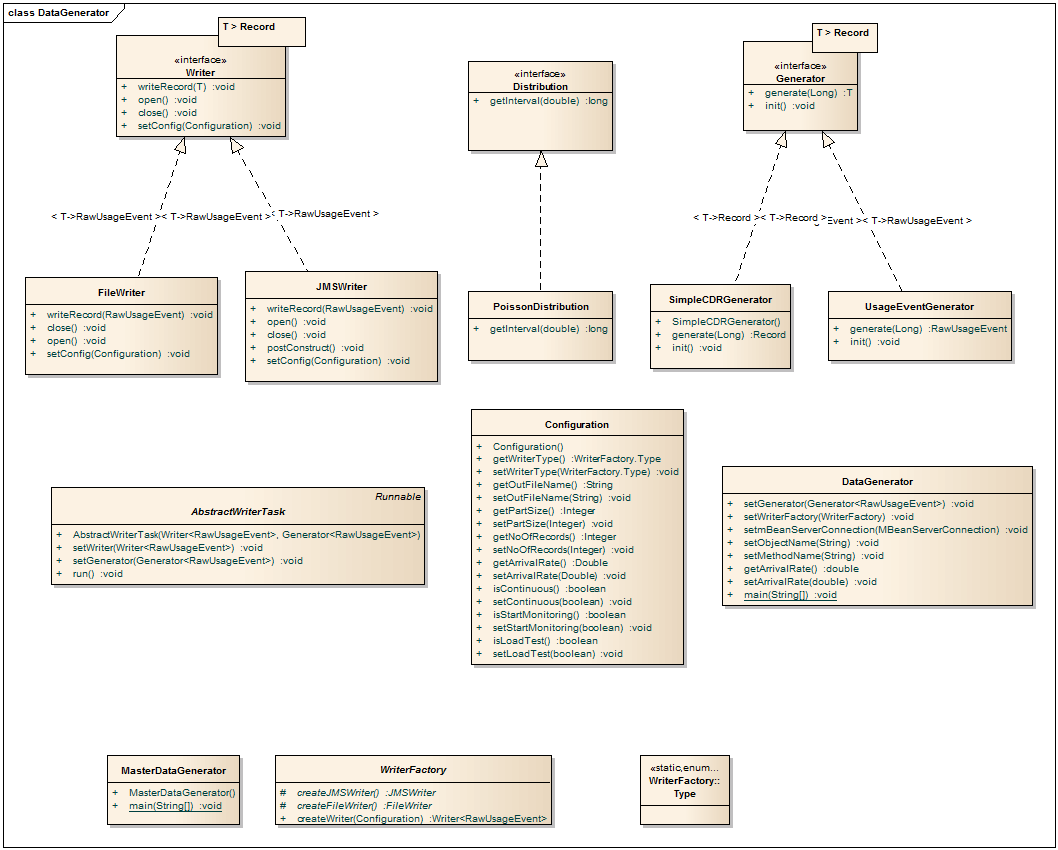
\includegraphics[width=\textwidth]{ch6_datagenerator_classdiagram}
	\caption{Datagenerator: Class diagram}
	\label{fig:ch5_datagenerator_classdiagram}
\end{figure}

\begin{itemize}
	\item Description of main classes
\end{itemize}

\subsubsection{Event Distribution}

\begin{itemize}
	\item Poisson Process
	\begin{itemize}
		\item Events occur continuously and independently of each other
		\item Exponentially distributed inter-arrival times
	\end{itemize}
\end{itemize}

\subsection{Sensors}

\subsubsection{QueueLengthSensor}

\begin{itemize}
	\item Base class JmxSensor
	\item Reads the current queue length of the ActiveMQ instance using JMX
\end{itemize}

\subsection{Controller}

\begin{itemize}
	\item ControllerStrategy Interface
\end{itemize}

\begin{lstlisting}[caption={ControllerStrategy Interface},label=listing:ch5_controller_strategy]
package com.jswiente.phd.performance.controller;

public interface ControllerStrategy {
	public Double getOutput(Double error);
}
\end{lstlisting}

\subsubsection{Simple Controller}

\subsubsection{PID Controller}

\begin{lstlisting}[caption={Implementation of PID Controller},label=listing:ch5_pid_controller]
public class PIDController implements ControllerStrategy {
	
	@Value("${controller.kp}")
	private Double kp;
	
	@Value("${controller.ki}")
	private Double ki;
	
	@Value("${controller.kd}")
	private Double kd;
	
	@Value("${controller.ta}")
	private Double ta;
	
	private Double errorSum = 0.0;
	private Double previousError = 0.0;

	public Double getOutput(Double error) {
		errorSum = errorSum + error;
		Double output = kp * error + ki * ta * errorSum + (kd * (error - previousError)/ta);
		previousError = error;
		return output;
	}

	//Setter methods removed for simplification...

}

\end{lstlisting}

\subsection{Actuator}

\begin{itemize}
	\item Interface Actuator
	\item AggregateSizeActuator
\end{itemize}
\begin{lstlisting}[caption={Actuator Interface},label=listing:ch5_actuator_interface]
package com.jswiente.phd.performance.actuator;

public interface Actuator<T> {

	public void setValue(T value);
}
\end{lstlisting}

\section{Evaluation}

\subsection{Test Environment}

\begin{itemize}
	\item Same test environment has been used as described in Section \ref{sec:ch4_test_environment}
\end{itemize}

\subsection{Test Design}

\subsubsection{Static Tests}

\subsubsection{Step Tests}

\subsubsection{Dynamic Tests}

\subsection{Results}

\section{Related Work}\label{sec:ch5_related_work}
\subsection{Adaptive Middleware}
Research on messaging middleware currently focusses on Enterprise Services Bus (ESB) infrastructure. An ESB is an integration plattform that combines messaging, web services, data transformation and intelligent routing to connect multiple heterogeneous services \citep{Chappell:2004jo}. It is a common middleware to implement the integration layer of an Service Oriented Architecture (SOA) and is available in numerous commercial and open-source packages.

Several research has been done to extend the static service composition and routing features of standard ESB implementations with dynamic capabilities decided at run-time, such as dynamic service composition \citep{Chang:2007aa}, routing \citep{Bai:2007aa} \citep{Wu:2008aa} \citep{Ziyaeva:2008aa} and load balancing \citep{Jongtaveesataporn:2010aa}.

Work to manage and improve the Quality of Service (QoS) of ESB and service-based systems in general is mainly focussed on dynamic service composition and service selection based on monitored QoS metrics such as throughput, availability and response time \citep{Calinescu:2011aa}. \cite{Gonzalez:2011} propose an adaptive ESB infrastructure to adress QoS issues in service-based systems which provides adaption strategies for response time degradation and service saturation, such as invoking an equivalent service, using previously stored information, distributing requests to equivalent services, load balancing and deferring service requests.

\subsection{Message Batching}
The adaption strategy of our middleware is to change the message aggregation size based on the current load of the system. Aggregating or batching of messages is a common approach to increase the throughput of a messaging system, for example to increase the throughput of total ordering protocols \citep{Friedman:1997aa} \citep{Friedman:2006aa} \citep{Romano:2012aa} \citep{Didona:2012aa}.


\subsection{Dynamic Scaling}
A different solution to handle infrequent load spikes is to automatically instantiate additional server instances, as provided by current Platform as a Service (PaaS) offerings such as Amazon EC2 \citep{ec2_autoscaling} or Google App Engine \citep{google_cloud_autoscaling}. While scaling is a common approach to improve the performance of a system, it also leads to additional operational and possible license costs. Of course, our solution can be combined with these auto-scaling approaches.

\subsection{Feedback Control of Computing Systems}

\section{Summary}\label{sec:ch5_summary}
In this paper, we have presented a middleware that is able to adapt itself to changing load scenarios by fluently shifting the processing type between single event and batch processing. The middleware uses a closed feedback loop to control the end-to-end latency of the system by adjusting the level of message aggregation depending on the current load of the system. Determined by the aggregation size of a messsage, the middleware routes a message to appropriate service endpoints, which are optimized for either single-event or batch processing.

To evaluate the proposed middleware concepts, we have implemented a prototype system and performed preliminary performance tests. The tests show that throughput and latency of a messaging system depend on the level of data granularity and that the throughput can be increased by increasing the granularity of the processed messages.

Next steps of our research are the implementation of the proposed middleware including the evaluation and tuning of different controller architectures, performance evaluation of the proposed middleware using the prototype and developing a conceptional framework containing guidelines and rules for the practitioner how to implement an enterprise system based on the adaptive middleware for near-time processing
